\documentclass[11pt]{article}
\usepackage[utf8]{inputenc}
\usepackage[T1]{fontenc}
\usepackage{lmodern}
\usepackage{geometry}
\usepackage[numbers,sort&compress]{natbib}
\usepackage{hyperref}
\usepackage{graphicx}
\usepackage{float}
\usepackage{amsmath,amssymb}
\usepackage{booktabs}
\usepackage{longtable}
\usepackage{enumitem}
\usepackage{microtype}
\usepackage{xcolor}
\geometry{margin=1in}

\hyphenpenalty=10000
\exhyphenpenalty=10000
\tolerance=2000
\emergencystretch=2em
\sloppy

\hypersetup{
  colorlinks=true,
  linkcolor=blue,
  citecolor=blue,
  urlcolor=blue
}

\title{A Reproducible Benchmark for Machine Learning \\
in Cross-Sectional Quantitative Trading \\
under Realistic Costs and Regime Shifts}
\author{Zhang Yuchen \\
  AI, Ethics and Society Programme, Faculty of Arts, \\
  The University of Hong Kong, Hong Kong SAR, China \\
  \texttt{u3663696@connect.hku.hk} \quad \texttt{georgekingsman030226@gmail.com}}
\date{}

\begin{document}
\maketitle

\begin{abstract}
Machine learning (ML) models for quantitative trading are routinely evaluated under conditions that inflate reported performance: costs are ignored, splits leak future information, and statistical significance is not tested.
We present \textbf{ML Trading Bench}, a unified evaluation protocol and open-source toolkit that applies walk-forward splitting with embargo, a configurable transaction-cost model, and rigorous statistical testing to a reproducible cross-sectional trading setting.
Using 50 US-listed ETFs over 2005--2024, we evaluate 9~models (linear, tree, and deep-learning families) plus 2~passive baselines across 5~cost scenarios, 4~market regimes, and multiple strategy hyperparameter configurations.

Our key findings challenge common claims in the literature:
(i)~all bootstrap 95\% confidence intervals on gross Sharpe ratios include zero;
(ii)~at 15\,bps one-way cost, every long-short strategy turns deeply negative;
(iii)~after Benjamini--Hochberg FDR correction, no ML-vs-ML pair is statistically distinguishable under the Diebold--Mariano test;
(iv)~strategy hyperparameters (rebalance frequency, portfolio concentration) shift Sharpe by $>$0.5---often more than model choice;
(v)~regime decomposition reveals that COVID-era volatility drives most headline results.

The full pipeline---from data download to 9~tables and 9~figures---runs in under 6~minutes with a single command (\texttt{python run\_all.py}).
Code, data scripts, and configuration are released under MIT license at
\url{https://github.com/georgekingsman/ml-trading-benchmark}.
\end{abstract}

\noindent\textbf{Keywords:}
quantitative trading;
machine learning benchmark;
reproducibility;
transaction costs;
regime analysis;
walk-forward evaluation;
statistical testing

\tableofcontents
\newpage

% ================================================================== %
\section{Introduction}
\label{sec:intro}

Machine learning is now central to quantitative trading, supporting signal discovery, portfolio construction, and execution under uncertainty and frictions~\citep{ref7,ref13,ref8}.
Yet a large fraction of reported ``alpha'' disappears once evaluation is made realistic.
Common pitfalls include: look-ahead leakage through naive train/test splits, omission of transaction costs, lack of statistical significance testing, and neglect of regime-dependent fragility~\citep{ref41,ref42,ref5}.

These evaluation gaps have practical consequences.
A model that appears to deliver Sharpe~1.0 in a zero-cost backtest may produce Sharpe~$-1.5$ once realistic turnover costs are applied.
A model comparison that appears significant may lose all significance after multiple-testing correction.
Without controlled benchmarks, practitioners and reviewers cannot distinguish genuine progress from evaluation artifacts.

\paragraph{Contributions.}
This paper makes three contributions:

\begin{enumerate}[leftmargin=1.6em]
  \item \textbf{A unified evaluation protocol} that combines walk-forward splitting with embargo, rolling z-score normalisation using only training data, and a configurable fee-plus-slippage cost model---designed to prevent the most common pitfalls that inflate reported performance.

  \item \textbf{A one-click reproducible toolkit}: the command \texttt{python run\_all.py} executes the full data$\to$train$\to$backtest$\to$report pipeline, producing 9~tables and 9~figures with zero manual intervention in under 6~minutes.

  \item \textbf{Systematic empirical evidence} on a realistic ETF universe: cost sensitivity analysis across 5~scenarios, per-regime performance decomposition across 4~market regimes, hyperparameter sensitivity studies (rebalance frequency, portfolio concentration), and rigorous statistical testing via bootstrap confidence intervals and the Diebold--Mariano test~\citep{ref_dm} with Benjamini--Hochberg FDR correction~\citep{ref_bh}.
\end{enumerate}

\paragraph{Paper organisation.}
Section~\ref{sec:related} reviews related work.
Section~\ref{sec:design} describes the benchmark design (universe, features, splits, cost model).
Section~\ref{sec:models} presents the model families and strategies.
Section~\ref{sec:evaluation} details the evaluation methodology and statistical tests.
Section~\ref{sec:results} reports results.
Section~\ref{sec:reproducibility} describes the reproducibility package.
Section~\ref{sec:discussion} discusses implications and limitations.


% ================================================================== %
\section{Related Work}
\label{sec:related}

\paragraph{ML for trading surveys.}
Several surveys review ML methods for financial prediction and trading~\citep{ref14,ref16}, reinforcement learning for portfolio management~\citep{ref7,ref10}, and deep learning for asset pricing~\citep{ref15}.
These works provide taxonomies and broad coverage but typically do not include reproducible benchmarks or systematic cost/regime analysis.

\paragraph{Quantitative trading platforms.}
Qlib~\citep{ref11} (Microsoft) provides an end-to-end quant research platform with data handling, model training, and backtesting for Chinese/US equities.
FinRL~\citep{ref81} focuses on reinforcement learning with a gym-style interface.
Both are powerful frameworks but are primarily designed for practitioners building new strategies, rather than for controlled evaluation of existing model families under varying cost and regime assumptions.

\paragraph{Evaluation methodology.}
De~Prado~\citep{ref42,ref5} introduced purged cross-validation and embargo-based splits to prevent leakage in financial ML.
The Diebold--Mariano test~\citep{ref_dm} is widely used for comparing forecast accuracy.
Benjamini and Hochberg~\citep{ref_bh} proposed FDR control for multiple hypothesis testing.
Harvey et al.~\citep{ref_harvey} argued that many reported trading ``factors'' are spurious due to multiple testing.
Our benchmark integrates these methodological innovations into a unified, automated pipeline.

\paragraph{Positioning.}
Unlike survey papers that prescribe best practices, our work \emph{demonstrates their consequences} in a concrete, reproducible setting.
Unlike trading platforms, our focus is on controlled evaluation rather than strategy development.
The closest analogue is a ``benchmark paper'' in the style of ImageNet~\citep{ref_imagenet} or GLUE~\citep{ref_glue} for NLP---adapted to the unique challenges of financial time series.


% ================================================================== %
\section{Benchmark Design}
\label{sec:design}

\subsection{Universe and Data}

We select 50 US-listed ETFs spanning equity sectors (SPY, QQQ, XLF, XLE, XLK, etc.), fixed income (TLT, IEF, HYG), commodities (GLD, USO), and currencies (UUP, FXE).
The ETF universe avoids individual-stock survivorship bias: all 50 ETFs remain listed throughout the full sample period (January 2005 to December 2024).
Daily OHLCV data are obtained from Stooq (primary; no API key, no rate limit) with yfinance as fallback.

\paragraph{Data statement.}
All data are freely available from public sources.
Stooq provides adjusted OHLCV without survivorship filtering.
We do not use point-in-time fundamental data; all features are derived from price and volume (see below).
Corporate actions (splits, dividends) are handled by the data provider's adjustment.
Missing data (delistings, holidays) are forward-filled for at most 5 days; tickers with $>$10\% missing days are excluded.

\subsection{Features and Labels}

We engineer 13 technical features per ticker per day:

\begin{itemize}[leftmargin=1.4em]
  \item \textbf{Returns}: 1-day, 5-day, 20-day log returns
  \item \textbf{Volatility}: 20-day and 60-day rolling standard deviation
  \item \textbf{Momentum}: 10-day and 20-day momentum (cumulative return)
  \item \textbf{RSI}: 14-day relative strength index
  \item \textbf{Moving-average ratios}: close/MA(10) and close/MA(50)
  \item \textbf{Volume}: 20-day volume ratio (current/rolling average)
  \item \textbf{Intraday range}: (high $-$ low) / close
\end{itemize}

All features are rolling z-score normalised using a \textbf{strictly trailing 252-day window}.
This is critical: normalisation statistics are computed only on past data, preventing any leakage of future distributional information.

The prediction target is the \textbf{5-day forward return} (cross-sectional; used for ranking, not regression accuracy).

\subsection{Walk-Forward Split with Embargo}

\begin{itemize}[leftmargin=1.4em]
  \item \textbf{Training}: June 2005 -- December 2016 (~12 years)
  \item \textbf{Validation}: January 2017 -- December 2019 (~3 years)
  \item \textbf{Test}: January 2020 -- December 2024 (~5 years)
  \item \textbf{Embargo}: 5 trading days at each boundary
\end{itemize}

The embargo gap removes potential label-overlap leakage between adjacent periods.
All hyperparameters are selected on the validation set; the test set is \textbf{never} used for model selection.
Figure~\ref{fig:timeline} illustrates the protocol.

\begin{figure}[H]
\centering
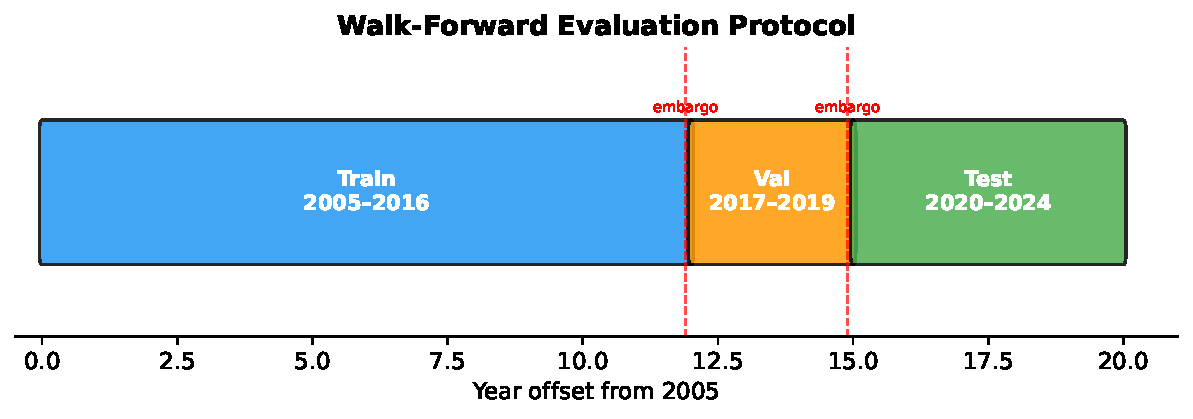
\includegraphics[width=0.92\textwidth]{../figs/bench_timeline.pdf}
\caption{Walk-forward evaluation protocol with embargo gaps. No information from downstream periods can influence upstream training or normalisation.}
\label{fig:timeline}
\end{figure}

\subsection{Cost Model}

Transaction costs are modelled as:
\begin{equation}
\text{cost}_t = (\text{fee} + \text{slippage}) \times \sum_i |\Delta w_{i,t}|,
\end{equation}
where $\Delta w_{i,t}$ is the weight change for asset $i$ at rebalance time $t$.
We evaluate five cost scenarios: 0, 5, 10, 15, and 25\,bps one-way (with an additional 5\,bps slippage).
This range spans from optimistic institutional settings to retail-level costs.


% ================================================================== %
\section{Models and Strategies}
\label{sec:models}

\subsection{Model Families}

We evaluate 9 models spanning three families discussed in the quantitative trading literature, plus 2 passive benchmarks:

\paragraph{Traditional ML (5 models).}
\begin{itemize}[leftmargin=1.4em]
  \item \textbf{Linear Regression} and \textbf{Ridge}: standard baselines with L2 regularisation.
  \item \textbf{Logistic Regression}: predicts direction probability, converted to a continuous signal.
  \item \textbf{Random Forest}: 200 trees, max depth 10.
  \item \textbf{LightGBM}: gradient-boosted trees with 500 rounds and early stopping on the validation set.
\end{itemize}

\paragraph{Deep Learning (2 models).}
\begin{itemize}[leftmargin=1.4em]
  \item \textbf{MLP}: 2-layer feedforward network (128--64 hidden units), ReLU activation, 50 epochs.
  \item \textbf{LSTM}: 2-layer LSTM (hidden dim 64, sequence length 20), 50 epochs.
\end{itemize}

\paragraph{Naive Strategies (2 baselines).}
\begin{itemize}[leftmargin=1.4em]
  \item \textbf{Momentum Baseline}: ranks assets by trailing 20-day return.
  \item \textbf{Mean Reversion Baseline}: ranks assets by negative 5-day return.
\end{itemize}

\paragraph{Ensemble.}
We construct a rank-average ensemble of all ML models: for each date, we compute the cross-sectional percentile rank of each model's prediction, then average across models.

\paragraph{Passive Benchmarks.}
\begin{itemize}[leftmargin=1.4em]
  \item \textbf{SPY Buy-and-Hold}: 100\% allocation to the S\&P~500 ETF.
  \item \textbf{Equal Weight (1/N)}: daily equal-weight allocation across all 50 ETFs.
\end{itemize}

These passive benchmarks incur zero turnover and serve as the ``minimum bar'' against which active strategies must be judged.

\subsection{Strategy Construction}

At each rebalance date (default: every 5 trading days), assets are ranked by predicted signal.
The \textbf{long-short strategy} goes long the top-$K$ and short the bottom-$K$ with equal weights ($\pm 1/K$ per leg; default $K=10$).
The \textbf{long-only variant} holds only the top-$K$ with equal weights.


% ================================================================== %
\section{Evaluation Methodology}
\label{sec:evaluation}

\subsection{Performance Metrics}

\begin{itemize}[leftmargin=1.4em]
  \item \textbf{CAGR}: compound annual growth rate (gross and net of costs)
  \item \textbf{Sharpe ratio}: annualised (gross and net), assuming zero risk-free rate
  \item \textbf{Maximum drawdown}: largest peak-to-trough decline
  \item \textbf{Calmar ratio}: CAGR / max drawdown
  \item \textbf{Hit rate}: fraction of positive-return days
  \item \textbf{Average turnover}: inferred from cost series
\end{itemize}

\subsection{Signal-Level Metrics}

\begin{itemize}[leftmargin=1.4em]
  \item \textbf{Information Coefficient (IC)}: daily cross-sectional Spearman rank correlation between predictions and realised 5-day returns.
  \item \textbf{ICIR}: IC divided by its standard deviation across days; measures signal stability.
\end{itemize}

\subsection{Bootstrap Confidence Intervals}

We compute 95\% confidence intervals on the gross Sharpe ratio via block bootstrap ($B=1{,}000$ resamples) to assess whether any model's performance is statistically distinguishable from zero.

\subsection{Diebold--Mariano Test with FDR Correction}

We apply the two-sided Diebold--Mariano (DM) test~\citep{ref_dm} pairwise across all $\binom{n}{2}$ model pairs using daily gross returns as the loss differential, with Newey--West HAC standard errors (bandwidth $h=5$).

\paragraph{Multiple testing correction.}
With $n=12$ models, we have $\binom{12}{2} = 66$ pairwise comparisons.
Testing each at $\alpha=0.05$ inflates the family-wise Type I error rate.
We apply the Benjamini--Hochberg (BH) procedure~\citep{ref_bh} to control the false discovery rate (FDR) at 5\%.
This is a one-line addition to the pipeline but significantly strengthens the statistical rigour of model comparisons.

\subsection{Regime Decomposition}

We partition the test period into four macro-regimes based on well-known market events:
\begin{enumerate}[leftmargin=1.6em]
  \item \textbf{COVID Crash}: February 2020 -- June 2020
  \item \textbf{Recovery}: July 2020 -- December 2021
  \item \textbf{Rate Hikes}: January 2022 -- December 2022
  \item \textbf{Normalisation}: January 2023 -- December 2024
\end{enumerate}

For each model, we report gross Sharpe within each regime to reveal whether headline performance is driven by a single extreme period.

\subsection{Hyperparameter Sensitivity}

We systematically vary two strategy hyperparameters that receive little attention in the literature:
\begin{itemize}[leftmargin=1.4em]
  \item \textbf{Rebalance frequency}: 1, 5, 10, 20 trading days
  \item \textbf{Portfolio concentration (top-$K$)}: 3, 5, 10, 15, 20 assets
\end{itemize}

This tests whether conclusions are robust to ``nuisance'' strategy parameters, or whether these parameters dominate model choice.


% ================================================================== %
\section{Results}
\label{sec:results}

\subsection{Main Results}

Table~\ref{tab:main} reports the core metrics on the test period (January 2020 -- December 2024).

\begin{table}[H]
\centering
\caption{Main benchmark results. Sharpe CI denotes the 95\% bootstrap confidence interval on the gross Sharpe ratio. IC and ICIR are computed cross-sectionally.}
\label{tab:main}
\footnotesize
\begin{tabular}{l r r r r r r r r}
\toprule
Model & \multicolumn{1}{c}{CAGR} & \multicolumn{1}{c}{Sharpe} & \multicolumn{1}{c}{Sharpe} & \multicolumn{1}{c}{Max DD} & \multicolumn{1}{c}{IC} & \multicolumn{1}{c}{ICIR} & \multicolumn{2}{c}{Sharpe 95\% CI} \\
      & \multicolumn{1}{c}{(g, \%)} & \multicolumn{1}{c}{(gross)} & \multicolumn{1}{c}{(net)} & \multicolumn{1}{c}{(\%)} & & & \multicolumn{1}{c}{lo} & \multicolumn{1}{c}{hi} \\
\midrule
\textit{BuyAndHold\_SPY} & \textit{14.86} & \textit{0.765} & \textit{0.765} & \textit{33.72} & \textit{---} & \textit{---} & \textit{$-$0.12} & \textit{1.68} \\
\textit{EqualWeight} & \textit{6.82} & \textit{0.515} & \textit{0.515} & \textit{26.32} & \textit{---} & \textit{---} & \textit{$-$0.39} & \textit{1.45} \\
\midrule
LogisticRegression  & 7.04  & 0.469 & $-$1.44 & 21.33 & 0.010 & 0.037 & $-$0.43 & 1.35 \\
LinearRegression    & 6.21  & 0.432 & $-$1.46 & 18.93 & 0.015 & 0.051 & $-$0.48 & 1.35 \\
RandomForest        & 4.47  & 0.372 & $-$1.56 & 28.55 & 0.005 & 0.019 & $-$0.56 & 1.29 \\
Ensemble            & 4.73  & 0.347 & $-$1.48 & 22.66 & 0.011 & 0.040 & $-$0.57 & 1.27 \\
MLP                 & 3.30  & 0.294 & $-$1.44 & 26.00 & 0.005 & 0.024 & $-$0.57 & 1.09 \\
LightGBM            & 3.34  & 0.290 & $-$1.51 & 24.02 & 0.007 & 0.028 & $-$0.65 & 1.20 \\
MomentumBaseline    & 0.67  & 0.134 & $-$0.69 & 39.44 & $-$0.011 & $-$0.036 & $-$0.75 & 1.01 \\
LSTM                & $-$3.53 & $-$0.167 & $-$2.00 & 25.95 & 0.009 & 0.042 & $-$1.07 & 0.74 \\
MeanReversion       & $-$4.69 & $-$0.134 & $-$0.97 & 44.77 & 0.011 & 0.036 & $-$1.01 & 0.75 \\
\bottomrule
\end{tabular}
\end{table}

\paragraph{Observations.}
\begin{enumerate}[leftmargin=1.6em]
  \item All models exhibit weakly positive cross-sectional IC ($\sim$0.005--0.015), confirming marginal predictive content.
  \item Every active strategy's gross Sharpe falls below SPY buy-and-hold (0.765) and most fall below equal-weight (0.515).
  \item At 15\,bps cost, all long-short strategies produce deeply negative net Sharpe ratios.
  \item \textbf{All bootstrap 95\% CIs include zero}---no model's gross performance is statistically distinguishable from zero at the 5\% level.
\end{enumerate}

\subsection{Cost Sensitivity}

Figure~\ref{fig:cost} plots net Sharpe against one-way transaction cost.
The ``alpha cliff'' is evident: even at 5\,bps, most models turn negative.

\begin{figure}[H]
\centering
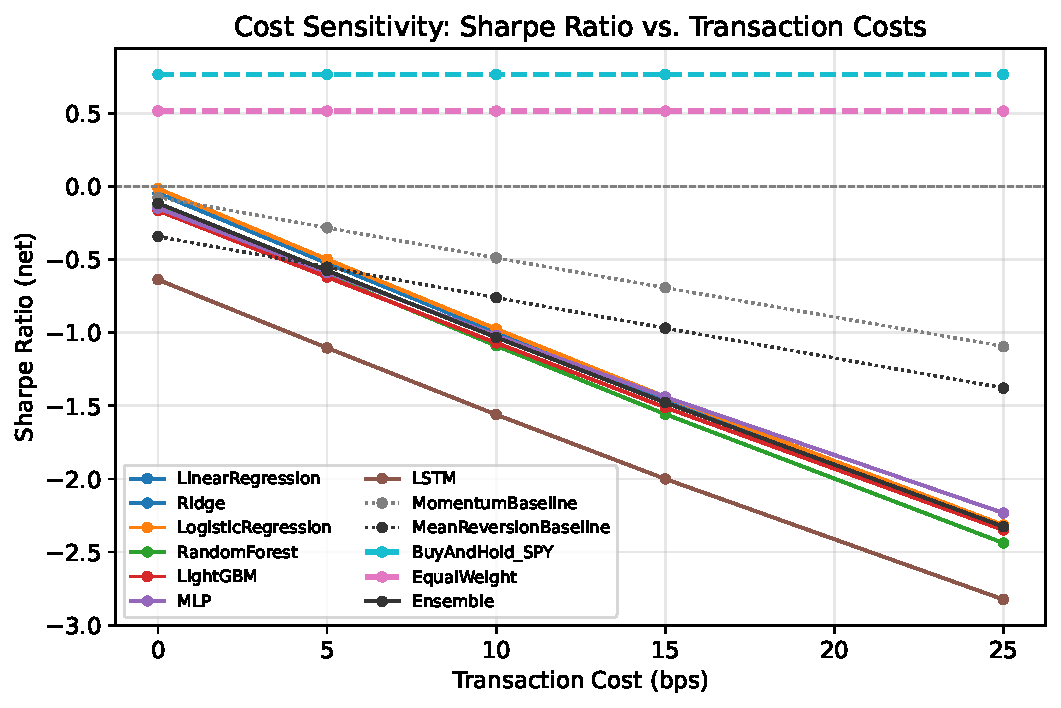
\includegraphics[width=0.80\textwidth]{../figs/bench_cost_sensitivity.pdf}
\caption{Net Sharpe ratio vs.\ one-way transaction cost (bps). Passive benchmarks are flat because they incur zero turnover. The steep decline illustrates the ``alpha cliff'': small costs erase small signals.}
\label{fig:cost}
\end{figure}

\subsection{Regime Analysis}

Table~\ref{tab:regime} decomposes performance across four regimes.

\begin{table}[H]
\centering
\caption{Gross Sharpe ratio by regime.}
\label{tab:regime}
\footnotesize
\begin{tabular}{l r r r r}
\toprule
Model & COVID Crash & Recovery & Rate Hikes & Normalisation \\
\midrule
BuyAndHold\_SPY       & $+$0.08   & $+$2.19  & $-$0.71 & $+$1.93 \\
EqualWeight           & $-$0.04   & $+$2.05  & $-$0.68 & $+$1.07 \\
LogisticRegression    & $+$0.74   & $+$1.47  & $+$0.69 & $-$0.53 \\
RandomForest          & $+$1.87   & $+$0.24  & $+$0.38 & $-$0.19 \\
LightGBM              & $+$1.41   & $+$0.54  & $+$0.23 & $-$0.30 \\
MLP                   & $+$1.21   & $+$0.42  & $+$0.17 & $+$0.05 \\
LSTM                  & $+$0.23   & $-$0.18  & $-$0.22 & $-$0.18 \\
Ensemble              & $+$1.31   & $+$0.86  & $+$0.47 & $-$0.57 \\
MomentumBaseline      & $+$1.02   & $+$0.88  & $-$1.44 & $-$0.19 \\
\bottomrule
\end{tabular}
\end{table}

\paragraph{Observations.}
Active models dramatically outperform buy-and-hold during the COVID crash (long-short benefits from elevated volatility and cross-sectional dispersion), but underperform in trending markets (recovery, normalisation).
This regime sensitivity is precisely the evaluation gap that headline Sharpe ratios hide.
Momentum collapses during rate hikes ($-$1.44), consistent with well-documented factor crashes.

\subsection{Hyperparameter Sensitivity}

Table~\ref{tab:sensitivity} reports gross Sharpe under varying rebalance frequencies and top-$K$ values.

\begin{table}[H]
\centering
\caption{Gross Sharpe ratio under different rebalance frequencies (days) and top-$K$ values.}
\label{tab:sensitivity}
\footnotesize
\begin{tabular}{l r r r r | r r r r r}
\toprule
 & \multicolumn{4}{c|}{Rebalance Frequency (days)} & \multicolumn{5}{c}{Top-$K$} \\
Model & 1 & 5 & 10 & 20 & 3 & 5 & 10 & 15 & 20 \\
\midrule
LogisticRegression & 0.66 & 0.47 & 0.15 & 0.34 & 0.95 & 1.03 & 0.47 & 0.60 & 0.58 \\
LightGBM           & 0.31 & 0.29 & 0.31 & 0.18 & $-$0.08 & 0.10 & 0.29 & 0.20 & 0.12 \\
MLP                & 0.31 & 0.29 & $-$0.16 & $-$0.67 & 0.55 & 0.42 & 0.29 & 0.38 & 0.22 \\
LSTM               & 0.63 & $-$0.17 & $-$0.29 & $-$0.82 & 0.35 & 0.16 & $-$0.17 & $-$0.08 & $-$0.26 \\
Ensemble           & 0.73 & 0.35 & 0.22 & 0.12 & 0.61 & 0.37 & 0.35 & 0.42 & 0.46 \\
\bottomrule
\end{tabular}
\end{table}

\paragraph{Observations.}
Daily rebalancing yields substantially higher gross Sharpe for most models (Ensemble: 0.73 vs.\ 0.35 at 5-day), but this comes with proportionally higher turnover---and therefore worse net performance.
More concentrated portfolios (smaller $K$) amplify signal quality: Logistic Regression achieves Sharpe~1.03 at $K=5$ versus 0.47 at $K=10$, but at higher idiosyncratic risk.
\textbf{These hyperparameters shift Sharpe by $>$0.5---more than the difference between model families.}
Yet they are rarely stress-tested in ML trading papers.

\subsection{Statistical Significance}

We apply the DM test~\citep{ref_dm} pairwise across all 12 models (66 pairs).

\paragraph{Raw results.}
At $\alpha = 0.05$, only \textbf{3 pairs} are significant, and all involve the passive SPY benchmark.
No ML-vs-ML comparison achieves significance.

\paragraph{After BH correction.}
Applying Benjamini--Hochberg FDR correction~\citep{ref_bh} at the 5\% level, the number of significant pairs remains at~3 (involving passives only).
No ML-vs-ML pair survives correction.

This result carries a stark implication: \textbf{model comparisons in the literature, when evaluated under proper cost and split protocols, may not be meaningfully distinguishable.}

\subsection{Long-Only Variant}

Table~\ref{tab:longonly} compares long-short and long-only strategies.

\begin{table}[H]
\centering
\caption{Long-short (LS) vs.\ long-only (LO) comparison at 15\,bps.}
\label{tab:longonly}
\footnotesize
\begin{tabular}{l r r r r r r}
\toprule
 & \multicolumn{3}{c}{Long-Short} & \multicolumn{3}{c}{Long-Only} \\
Model & Sharpe(g) & Sharpe(n) & CAGR(g,\%) & Sharpe(g) & Sharpe(n) & CAGR(g,\%) \\
\midrule
LogisticRegression & 0.47 & $-$1.44 & 7.04 & 0.68 & $-$0.35 & 10.57 \\
LightGBM           & 0.29 & $-$1.51 & 3.34 & 0.65 & $-$0.13 & 10.55 \\
MLP                & 0.29 & $-$1.44 & 3.30 & 0.62 & $-$0.19 & 9.88 \\
LSTM               & $-$0.17 & $-$2.00 & $-$3.53 & 0.22 & $-$0.54 & 2.44 \\
Ensemble           & 0.35 & $-$1.48 & 4.73 & 0.65 & $-$0.34 & 10.19 \\
BuyAndHold\_SPY    & 0.77 & 0.77 & 14.86 & --- & --- & --- \\
\bottomrule
\end{tabular}
\end{table}

Long-only consistently produces higher gross Sharpe (e.g., LightGBM: 0.65 vs.\ 0.29) because it captures the long-run equity premium rather than relying solely on cross-sectional spread.
This suggests that, for most ML signals in this setting, the short leg destroys more value than it creates.

\subsection{Equity Curves}

Figure~\ref{fig:equity} shows cumulative gross returns with a drawdown subplot and regime shading.

\begin{figure}[H]
\centering
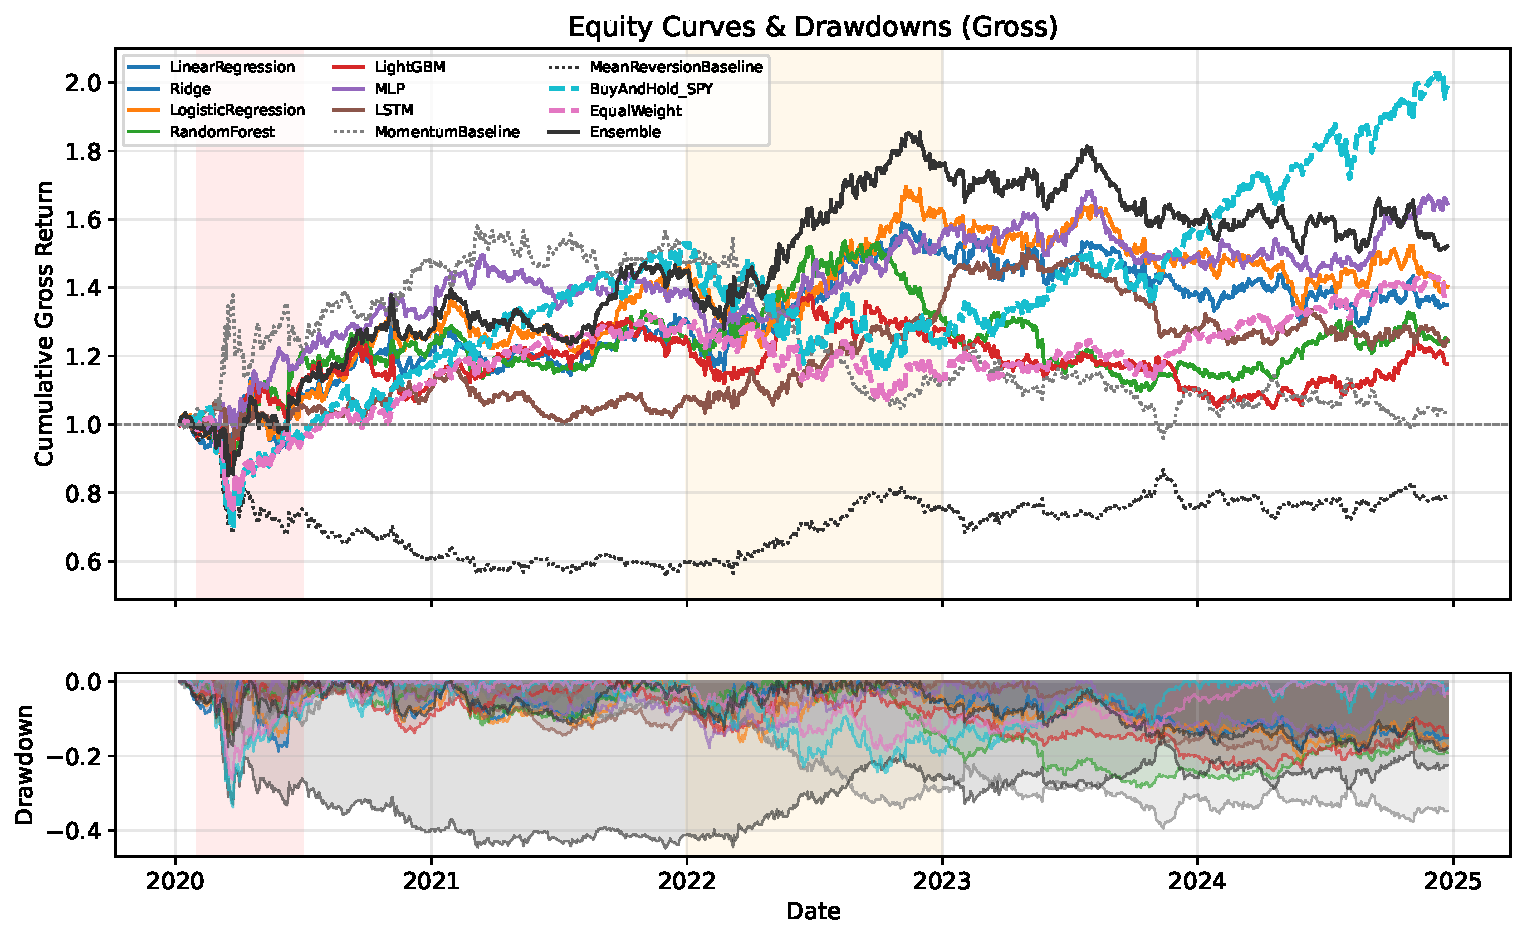
\includegraphics[width=0.95\textwidth]{../figs/bench_equity_curves.pdf}
\caption{Cumulative gross returns with drawdown subplot. Shaded bands: COVID crash (red), rate hikes (orange). Passive benchmarks shown as dashed lines.}
\label{fig:equity}
\end{figure}


% ================================================================== %
\section{Reproducibility Package}
\label{sec:reproducibility}

\subsection{Pipeline Overview}

The full benchmark is executed via:
\begin{verbatim}
    pip install -r requirements.txt
    python run_all.py
\end{verbatim}

This runs 13 sequential steps: data download, feature engineering, walk-forward split, model training, backtesting (long-short + long-only + passives), IC/ICIR/bootstrap CI, regime analysis, feature importance, ensemble construction, DM test with BH correction, rebalance sensitivity, top-$K$ sensitivity, and report generation.

\subsection{Runtime and Environment}

\begin{itemize}[leftmargin=1.4em]
  \item \textbf{Runtime}: $\sim$6 minutes on Apple M-series (M2, 16\,GB RAM)
  \item \textbf{Python}: $\geq$ 3.10
  \item \textbf{Key dependencies}: pandas, scikit-learn, LightGBM, PyTorch, statsmodels
  \item \textbf{Random seed}: fixed at 42 for full reproducibility
  \item \textbf{Data}: freely available from Stooq (no API key required)
\end{itemize}

\subsection{Output}

The pipeline produces:
\begin{itemize}[leftmargin=1.4em]
  \item \textbf{9 tables}: main results, cost sensitivity, regime analysis, feature importance, long-only comparison, DM test (raw + BH-corrected), rebalance sensitivity, top-$K$ sensitivity (CSV + \LaTeX)
  \item \textbf{9 figures}: walk-forward timeline, cost sensitivity curves, equity curves, ranking heatmap, feature importance, regime bars, rebalance sensitivity, top-$K$ sensitivity, DM heatmap (PDF)
  \item \textbf{JSON summary}: all numerical metrics in machine-readable format
\end{itemize}

\subsection{Code and License}

All code is released under MIT license at \url{https://github.com/georgekingsman/ml-trading-benchmark}.
The repository includes \texttt{REPRODUCIBILITY.md} (step-by-step instructions), \texttt{ENVIRONMENT.md} (platform notes), and \texttt{CITATION.cff} (machine-readable citation).


% ================================================================== %
\section{Discussion and Limitations}
\label{sec:discussion}

\subsection{Key Takeaways}

The benchmark yields several implications that we believe are generalisable beyond this specific setting:

\begin{enumerate}[leftmargin=1.6em]
  \item \textbf{The ``alpha cliff'' is real}: even modest costs ($\sim$5--15\,bps) erase the small predictive edge of ML models in a long-short ETF setting. Papers that report only gross metrics significantly overstate practical value.

  \item \textbf{Passive benchmarks must be reported}: without SPY buy-and-hold and equal-weight baselines, a reader cannot judge whether ML adds value beyond the equity risk premium.

  \item \textbf{Bootstrap CIs include zero for all models}: this underscores the need for statistical testing, not just point estimates.

  \item \textbf{Regime decomposition reveals hidden fragility}: models that look good on average may be entirely driven by one extreme period (e.g., COVID volatility).

  \item \textbf{Strategy hyperparameters dominate model choice}: rebalance frequency and portfolio concentration shift Sharpe by $>$0.5, often more than the difference between model families.

  \item \textbf{Multiple testing matters}: after BH-FDR correction, no ML-vs-ML pair is distinguishable, reinforcing the need for correction when comparing many models.

  \item \textbf{Model ensembling helps stability but not magnitude}: rank-average ensembles achieve middle-of-pack performance, suggesting that combining weak signals does not create strong ones in this regime.
\end{enumerate}

\subsection{Implications for the Research Community}

Our results do not imply that ML is useless for trading.
Rather, they demonstrate that \textbf{evaluation methodology matters as much as model architecture}, and that the gap between ``looks good in a backtest'' and ``is statistically and economically significant'' is larger than commonly acknowledged.

We recommend that future ML trading papers:
\begin{itemize}[leftmargin=1.4em]
  \item Report net performance under at least two cost scenarios
  \item Include passive benchmarks (buy-and-hold, equal-weight)
  \item Provide bootstrap CIs or equivalent statistical tests on key metrics
  \item Apply multiple-testing correction when comparing $>$2 models
  \item Report regime-conditional performance
  \item Release reproducible code
\end{itemize}

\subsection{Limitations}

\begin{enumerate}[leftmargin=1.6em]
  \item \textbf{Daily frequency only}: the benchmark does not cover intraday or tick-level strategies, where different evaluation challenges arise.
  \item \textbf{ETFs only}: individual stocks introduce survivorship bias and liquidity heterogeneity that our ETF universe avoids; results may differ.
  \item \textbf{Technical features only}: we do not include fundamental, alternative, or text-based features, which may provide stronger signals in practice.
  \item \textbf{Simplified cost model}: our fee-plus-slippage model does not account for market impact (price displacement from large orders), which is relevant for institutional-scale strategies.
  \item \textbf{Single data period}: while we test across regimes within 2020--2024, the out-of-sample window is one contiguous period. A multi-fold walk-forward design would be stronger but computationally more expensive.
  \item \textbf{Linear cost model}: costs are proportional to turnover; in practice, costs are non-linear in order size and depend on market conditions.
\end{enumerate}

\subsection{Future Work}

Natural extensions include:
(i)~expanding to individual stocks with survivorship-free data (e.g., CRSP);
(ii)~adding fundamental and alternative-data features;
(iii)~incorporating market impact models;
(iv)~multi-fold walk-forward evaluation;
(v)~including reinforcement learning agents;
and (vi)~adding intraday/LOB evaluation protocols.

\section{Conclusion}

We have presented ML Trading Bench, a unified evaluation protocol and toolkit that applies rigorous, cost-aware, regime-sensitive evaluation to cross-sectional ML trading strategies on a reproducible 50-ETF universe.
Our systematic evidence demonstrates that (i)~transaction costs eliminate all apparent alpha in a long-short setting, (ii)~no model achieves statistically significant gross performance, (iii)~strategy hyperparameters dominate model choice, and (iv)~headline results are fragile to regime decomposition.

The full pipeline runs in under 6 minutes with a single command, producing 9~tables and 9~figures.
We hope this benchmark serves as a useful starting point for more rigorous evaluation of ML methods in quantitative finance.


% ================================================================== %
\section*{Data Availability Statement}

All data used in this study are freely available from public sources (Stooq, yfinance).
No proprietary or restricted-access datasets are used.
The complete pipeline to download, process, and evaluate the data is available at
\url{https://github.com/georgekingsman/ml-trading-benchmark}.


\section*{Acknowledgments}
The author thanks colleagues at the University of Hong Kong for helpful discussions on quantitative trading systems and ML evaluation methodology.
This research did not receive any specific grant from funding agencies in the public, commercial, or not-for-profit sectors.

\subsection*{Declaration of Generative AI and AI-assisted Technologies in the Writing Process}
During the preparation of this work the author used AI-assisted tools to help with code development and literature review. After using these tools, the author reviewed and edited all content and takes full responsibility for the content of the published article.

\bibliographystyle{plainnat}
\bibliography{references_eswa_core60_filled}

\end{document}
